\documentclass[0-suturing.tex]{subfiles}
\begin{document}

%==START SECTION==============================
\section{Problem Formulation}
\label{sec:problem}
%=============================================
\
Well established manual suture techniques lay the foundation for robotic suturing. In order to complete an independent surgical suture, several components must be preplanned. First, the needle
must enter and exit the tissue in the proper locations and
orientations. Secondly, the needle path must not put any
unnecessary stress on the tissue. Finally, the needle must be
able to react to any unforeseen obstacles that might impede
the needle’s path.
The challenges in learning to suture are difficulty in needle pose estimation, modelling of needle-tissue interaction and creating trajectory plans for robust long-horizon execution. 

% warp the reference needle trajectory
% the reference trajectory is the goal and we want to use motion planning to generate a new trajectory that is close to the reference but minimizes some objective
% incorporate grasp uncertainty into motion plan
% use belief space planning to generate more robust needle trajectory 
\subsection{Suture placement}
The surgeon provides as input a desired suturing line through robotic tele-operation by tracing the tip of the robot's tool through the desired
suturing channel. Let $\mathcal{M} = [M_1, M_2, \ldots, M_D]$ be the discretized trajectory recorded by the system. The surgeon also provides a desired needle bite length $l$, desired bite depth $d$, and a stitch separation $w$.
The full input to our system then is $S,l,d,w$.
Our system outputs an optimal needle size for the given task and  a finite state machine that uses closed loop sensor feedback to autonomously perform a continuous suture. 

We first describe how needle entry and exit points can be generated from surgeon input. Each way point $S_t$ in the desired suturing line can be parametrized by $S_t \in \mathbb{R}^3$, a 3D point. We fit a cubic spline the the series of points to estimate the suturing line. The line is re-sampled such that the distance between each point is $w$ to generate the centers for each stitch in the suture. This can be formalized as the series of points $\mathcal{L} = [L_1, L_2, \ldots, L_F] $ where $ \|L_{i+1} - L_{i}\|_2 = w, \forall i \in [0, \dots, F-1]$. At each stitch center we can generate entry and exit points using equidistant points on opposite sides of the spline.
For each pair of entry and exit points, we developed a motion planning formulation to generate needle trajectories through the tissue.

\subsection{Needle Positioning and Insertion}
The needle's trajectory through the tissue can be discretized into time intervals. Given the entry point of the needle $p_i$, the exit point of the needle $p_f$, we would like to plan a needle motion plan between the two points. Based on the desired bite depth of the stitch, we can generate an avoidance volume below and and above the trajectory. By avoiding collisions with these volumes, we can generate trajectories that allow for successful tissue apposition.



\begin{figure}[t]
\centering
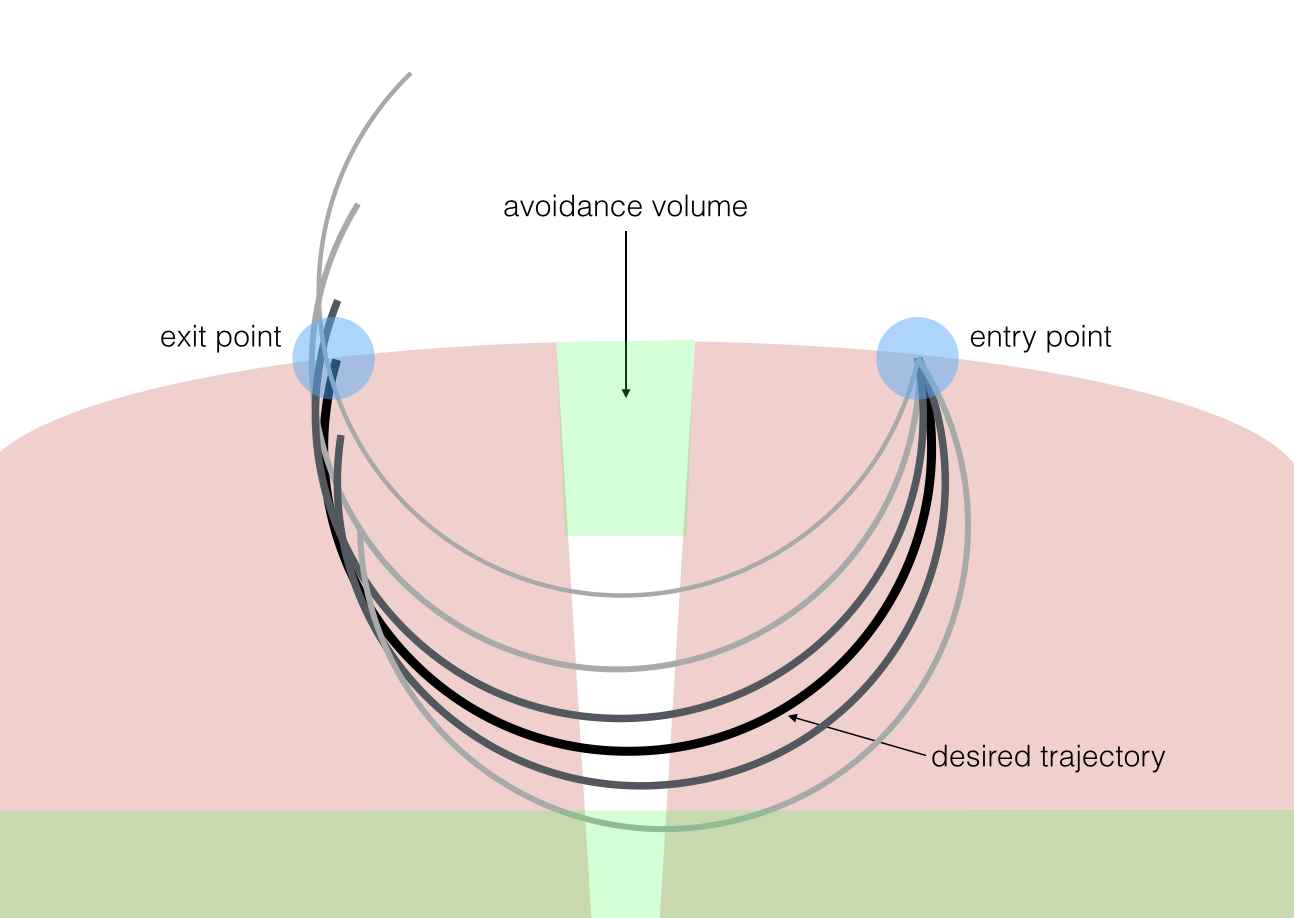
\includegraphics[width=0.85\linewidth]{figures/problem_image.jpg}
% \vspace{-5pt}
\caption{\todo{Placeholder} The is an illustration of a simulated trajectory as it is planned for a given set of parameters.}
\label{fig:toyEx}
\vspace{-15pt}
\end{figure}


\noindent{\textbf{Input:}}\\
We 
Avoidance volume: $\mathcal{O}$ \\
Desired entry point: $p_i$ \\
Desired exit point: $p_f$ \\

\noindent{\textbf{Output:}}\\


\noindent{\textbf{Assumptions:}}\\
- homogeneous tissue\\
- no FEA and tissue interaction model is used to model 
% \noindent{ \textbf{Optimization:}}\\

% some $\Delta$ values to very large numbers while others to zero, resulting 
\subsection{Evaluation Metric}
Performance of closed loop suturing will be measured by\\
- accuracy of needle tracking \\
- accuracy of one throw suturing \\
- accuracy of hand-off \\
- robustness to multi-throw suturing.
\todo{flesh out}


\begin{figure}[!t]
\centering
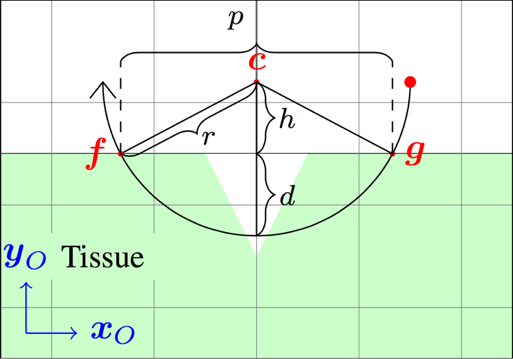
\includegraphics[width=0.8\linewidth]{figures/Schematic}
% \vspace{-5pt}
\caption{\todo{Placeholder} This figure illustrates the notation used in the the optimization problem \todo{refer}}
\label{fig:notation}
\vspace{-10pt}
\end{figure}


%==START SECTION==============================
% \subsection{Our Approach}
%==START SECTION==============================
\section{Proposed Algorithm}
\label{sec:approach}
%============================================
Overview plus block diagram \\

Trajectory Optimization
We use sequential quadratic programming to solve our nonlinear constrained optimization problem
Planning directly in SE(3) is hard
Convex opt works well in flat euclidean spaces
Possible pose representations:
3D+YPR
good: minimal state representation
bad: discontinuities in YPR, gimbal lock
3D + quaternions, 4x4 homogeneous matrix
good: jacobians are always well defined, quaternion work well in many cases
bad: lots of free variables (optimization can get stuck moving along degenerate solutions)
Better solution: optimize on the manifold using the lie algebra (note: used by others as well)
for each iteration of the optimization create a local coordinate parameterization
take gradient steps in $\mathfrak{se}$(3)
convert solution back to SE(3)
repeat for each iteration


\end{document}
